\documentclass[11pt]{article}

\usepackage{bm}
\usepackage[utf8]{inputenc}
\usepackage{array}
\usepackage{booktabs}   % For improved table formatting
\usepackage{tabulary}   % For tables with adjustable column widths
\usepackage{caption}
\usepackage{amsmath}
\usepackage{amssymb}
\usepackage{array}
\usepackage{tabularx}
\usepackage{xcolor}

\usepackage{enumitem}

\usepackage{pgfplots} % For creating graphs and plots
\pgfplotsset{compat=1.17} % Compatibility setting for pgfplots
\usepackage{graphicx} % For including graphics
\usepackage{float} % Helps to place figures and tables at precise locations
\usepackage{caption}
\usepackage{subcaption}

\let\oldemptyset\emptyset
\let\emptyset\varnothing

% Setting up the margins:
\usepackage[a4paper, total={6in, 10in}]{geometry}

\begin{document}

\title{Hypothesis Testing for One Proportion}
\author{POL 501}
\date{}
\maketitle

\section*{Introduction}

The goal of hypothesis testing is to assess whether the data we observe provide enough evidence to support a specific claim about a population parameter. In this note, we will formally derive and explain the process of hypothesis testing for a single population proportion. We start from the basic principles of probability and statistical inference, building toward the final test and its interpretation.

\section*{Purpose of Hypothesis Testing}

The fundamental purpose of hypothesis testing is to make decisions about population parameters based on sample statistics. It's a method of inferential statistics designed to test the validity of a claim, hypothesis, or model about a population using sample data. The aim is not just to ascertain the likelihood of a claim being true but to quantify the evidence against a null hypothesis (\( H_0 \)) in favor of an alternative hypothesis (\( H_1 \)).

The hypothesis testing framework is built upon the premise of examining whether the observed data would be very unlikely were the null hypothesis true. This approach closely aligns with the falsification principle in the philosophy of science. By testing whether the data contradict \( H_0 \) sufficiently to reject it, we make a probabilistic judgment about the tenability of our initial assumption.

\section*{Step 1: Setting Up the Hypothesis}

\subsection*{Definition: Hypothesis}
In statistics, a hypothesis is a claim or statement about a population parameter, such as a proportion \( p \). Hypothesis testing allows us to evaluate whether observed data is consistent with a hypothesis.

\subsubsection*{Types of Hypotheses}
Hypothesis tests involve two types of hypotheses:
\begin{itemize}
    \item \textbf{Null Hypothesis} (\( H_0 \)): This is the default hypothesis, representing no effect or no difference. For a proportion test, the null hypothesis states that the population proportion \( p \) is equal to some specified value \( p_0 \).
    \[
    H_0: p = p_0
    \]
    \item \textbf{Alternative Hypothesis} (\( H_1 \) or \( H_a \)): This is the hypothesis that we aim to gather evidence in favor of. It is a statement that the population proportion differs from \( p_0 \) in a specified direction (or in any direction if it’s a two-tailed test).
    \[
    H_a: p \neq p_0 \quad \text{(two-tailed)}
    \]
    or
    \[
    H_a: p > p_0 \quad \text{or} \quad H_a: p < p_0 \quad \text{(one-tailed)}
    \]
\end{itemize}

\subsection*{Example}
Suppose we want to test whether a newly implemented policy influenced voter approval of the President, currently assumed to be 60\%. We set up our hypotheses as follows:
\[
H_0: p = 0.60 \quad \text{and} \quad H_a: p \neq 0.60
\]
where \( p \) represents the true proportion of approval in the population.

To help understand the null hypothesis (\( H_0 \)) and the alternative hypothesis (\( H_1 \) or \( H_a \)), let's break it down non-technically:

\begin{itemize}
    \item \textbf{Null Hypothesis (\( H_0 \))}: Think of this as the ``status quo" or the assumption that nothing has changed. In our example, \( H_0: p = 0.60 \) means that we believe the true proportion of approval is \emph{still 60\%}. We use this as the baseline, and we're basically saying, ``Let's assume things haven't changed until we find convincing evidence otherwise."
    \item \textbf{Alternative Hypothesis (\( H_a \))}: This is the \emph{claim that something has changed}. In this case, \( H_a: p \neq 0.60 \) suggests that the proportion of approval might be \emph{different from 60\%}. It doesn't matter if it's higher or lower—just that it's not 60\%.
    \item \textbf{How to Interpret \( H_0 \) and \( H_a \)}:
    \begin{itemize}
        \item We start by assuming \( H_0 \) is true (i.e., approval is still 60\%).
        \item We then look at our data and ask, ``Is this data surprising enough to reject \( H_0 \)?"
        \item If the data is typical for 60\% approval (i.e., not surprising), we \emph{do not reject \( H_0 \)}. If the data is very different (i.e., surprising), we might \emph{reject \( H_0 \)} and conclude that \( H_a \) is more plausible.
    \end{itemize}
\end{itemize}

Essentially, \( H_0 \) is the ``nothing changed" hypothesis, and \( H_a \) is the ``something is different" hypothesis. The decision depends on whether our observed data is consistent with \( H_0 \) or if it falls into a region that suggests something else is going on (the \( H_a \) region).

\section*{Step 2: Understanding Sampling Distributions}

\subsection*{Probability and Random Variables}

Probability theory starts with the concept of a \textbf{probability space}, which consists of a sample space \( \Omega \), a set of events \( \mathcal{F} \), and a probability measure \( P \). Events are subsets of \( \Omega \) and \( P \) assigns a probability to each event, meeting the requirements:
\begin{itemize}
  \item \( P(A) \geq 0 \) for all \( A \in \mathcal{F} \)
  \item \( P(\Omega) = 1 \)
  \item If \( A_1, A_2, \ldots \) are disjoint (i.e., \( A_i \cap A_j = \emptyset \) for \( i \neq j \)), then \( P\left(\bigcup_{i=1}^\infty A_i\right) = \sum_{i=1}^\infty P(A_i) \)
\end{itemize}

A \textbf{random variable} \( X \) is a function from \( \Omega \) to the real numbers \( \mathbb{R} \), which is measurable with respect to \( \mathcal{F} \).

\subsection*{Distribution of Random Variables}

For a discrete random variable (such as a proportion in a binomial distribution), its distribution is described by a \textbf{probability mass function (PMF)}, which gives the probability that the random variable takes any specific value.

\subsubsection*{Example: The Binomial Distribution}
If \( S_n \) is the number of successes in \( n \) independent Bernoulli trials with success probability \( p \), then \( S_n \) follows a binomial distribution \( \text{Bin}(n, p) \) with PMF given by:
\[
P(S_n = k) = \binom{n}{k} p^k (1-p)^{n-k}
\]
for \( k = 0, 1, 2, \ldots, n \).

\subsection*{Estimation and the Law of Large Numbers}

From a theoretical perspective, the proportion \( \hat{p} = S_n/n \), where \( S_n \sim \text{Bin}(n, p) \), is an estimator of \( p \). By the law of large numbers, \( \hat{p} \) converges in probability to \( p \) as \( n \rightarrow \infty \), that is:
\[
\hat{p} \xrightarrow{P} p
\]

\subsection*{Central Limit Theorem (CLT)}

For large \( n \), the distribution of \( \hat{p} \) is approximately normal due to the CLT, which states that:
%\[\sqrt{n} \left(\hat{p} - p\right) \xrightarrow{d} \mathcal{N}\left(0, p(1-p)\right)\]
This implies:
\[
\hat{p} \approx \mathcal{N}\left(p, \frac{p(1-p)}{n}\right)
\]

\subsection*{Sampling Distribution of the Sample Proportion \( \hat{p} \)}

Recall that for a large sample size \( n \), the sample proportion \( \hat{p} = \frac{S_n}{n} \), where \( S_n \) is the sum of \( n \) Bernoulli trials, can be approximated by a normal distribution. Specifically:
\[
\hat{p} \sim N\left(p, \frac{p(1-p)}{n}\right)
\]
If we assume \( H_0 \) is true, then \( p = p_0 \), and the distribution of \( \hat{p} \) under \( H_0 \) is approximately:
\[
\hat{p} \sim N\left(p_0, \frac{p_0(1-p_0)}{n}\right)
\]
This distribution serves as our \textbf{reference distribution} for making probability-based decisions regarding \( H_0 \).

\section*{Step 3: Calculating the Test Statistic}

To quantify the difference between the observed sample proportion \( \hat{p} \) and the hypothesized proportion \( p_0 \), we compute a test statistic. 

\subsubsection*{Definition: Test Statistic}
The test statistic is a measure that standardizes the observed difference between the sample proportion and the hypothesized proportion under \( H_0 \). This standardization allows us to reference the standard normal distribution.

The test statistic for a hypothesis test on one proportion is given by:
\[
Z = \frac{\hat{p} - p_0}{SE(p_0, n)} = \frac{\hat{p} - p_0}{\sqrt{\frac{p_0(1-p_0)}{n}}}
\]
where:
\begin{itemize}
    \item \( \hat{p} \) is the observed sample proportion,
    \item \( p_0 \) is the hypothesized population proportion,
    \item \( n \) is the sample size.
    \item $SE(p_0, n)$ is the standard error of the sample proportion of sample size $n$, under the null hypothesis ($H_0: p=p_0$).
\end{itemize}


\subsection*{Intuition Behind the Test Statistic}

The test statistic \( Z \) measures how far the observed sample proportion \( \hat{p} \) is from the hypothesized proportion \( p_0 \), scaled by the standard error. A larger \( |Z| \) indicates a greater discrepancy between \( \hat{p} \) and \( p_0 \), relative to what we would expect under \( H_0 \) due to random sampling variability.

\section*{Step 4: Determining the Rejection Region}

\subsection*{Significance Level and Critical Value}
The \textbf{significance level} \( \alpha \) represents the probability of rejecting \( H_0 \) when it is actually true (Type I error). Common choices for \( \alpha \) are 0.05 or 0.01, meaning we accept a 5\% or 1\% risk of a Type I error.

\textbf{Mathematical Foundation and Significance Level (\( \alpha \))}

The significance level \( \alpha \) reflects the threshold of rejecting the null hypothesis, which we determine based on the probability of observing a test statistic at least as extreme as the one computed from the data, assuming \( H_0 \) is true. Mathematically, it's defined as:
\[
P(\text{Type I Error}) = P(\text{Reject } H_0 \mid H_0 \text{ is true}) = \alpha
\]
A common choice for \( \alpha \) is 0.05, indicating a 5\% risk of incorrectly rejecting \( H_0 \). This parameter is chosen to balance between making erroneous inferences and being overly cautious about rejecting the null hypothesis.

\noindent  \textbf{Type I Error (False Positive)}:
\begin{itemize}
  \item Occurs when \( H_0 \) is incorrectly rejected.
  \item Probability is controlled by \( \alpha \).
\end{itemize}

\noindent \textbf{Type II Error (False Negative)}:
\begin{itemize}
  \item Occurs when \( H_0 \) is not rejected, but \( H_1 \) is true.
  \item Denoted by \( \beta \), and \( 1 - \beta \) is the power of the test, the probability of correctly rejecting \( H_0 \) when \( H_1 \) is true.
\end{itemize}

The interplay between \( \alpha \) and \( \beta \) focuses on the risks we are willing to accept in the hypothesis testing procedure. Minimizing both errors simultaneously is often challenging, leading to a trade-off where reducing one increases the other.

\textbf{Intuition}. The significance level (\( \alpha \)) and critical value help us decide whether the evidence in our data is strong enough to reject the null hypothesis. Let's think of \( \alpha \) as our threshold for ``how much risk of being wrong we're willing to accept." For example, if we set \( \alpha = 0.05 \), it means we're willing to accept a 5\% chance of mistakenly rejecting the null hypothesis when it is actually true (this is called a Type I error). 

The critical value is the specific point in the distribution of our test statistic beyond which we reject the null hypothesis. In a two-tailed test with \( \alpha = 0.05 \), the critical value for the standard normal distribution is roughly 1.96 in both directions. This means that if our test statistic \( Z \) falls beyond +1.96 or below -1.96, it indicates that the observed sample proportion is unlikely to have happened by random chance alone if the null hypothesis were true. Essentially, these critical values define the boundaries of the ``rejection region," and if our test statistic falls within this region, we have enough evidence to reject \( H_0 \).

\subsection*{Visual Interpretation with a Z-Score Graph}

To deepen our understanding of how hypothesis testing quantifies the unlikelihood of observed data under the null hypothesis (\( H_0 \)), it's useful to visualize what it means for data to be ``unlikely" when \( H_0 \) is presumed true. We focus on the case where the sample proportions are approximately normally distributed, a common scenario in large samples due to the Central Limit Theorem.

\begin{center}
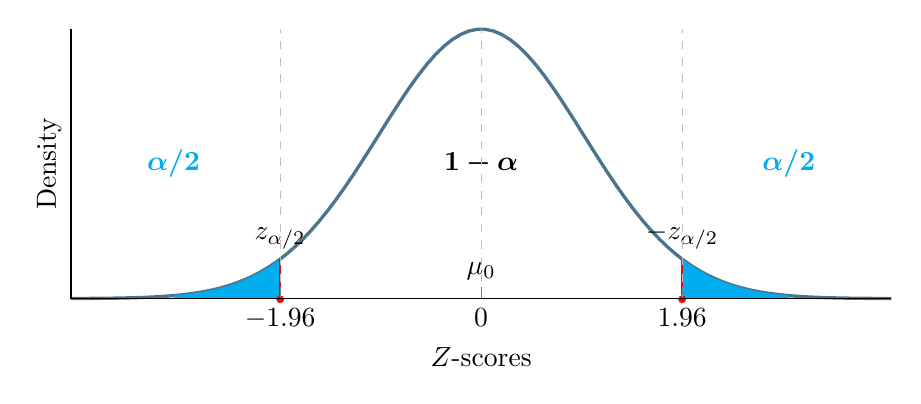
\begin{tikzpicture}
    \begin{axis}[
        samples=100,
        domain=-4:4,
        axis lines*=left,
        xlabel=$Z$-scores,
        ylabel={Density},
        height=5cm,
        width=12cm,
        xtick={-1.96, 0, 1.96},
        ytick=\empty,
        enlargelimits=false,
        clip=false,
        axis on top,
        grid=major,
        grid style={dashed}
    ]
        \addplot [very thick,cyan!50!black] {exp(-x^2/2) / sqrt(2*pi)};
        \addplot [fill=cyan, draw=none, domain=-3:-1.96] {exp(-x^2/2) / sqrt(2*pi)} \closedcycle;
        \addplot [fill=cyan, draw=none, domain=1.96:3] {exp(-x^2/2) / sqrt(2*pi)} \closedcycle;
        \node[pin={[pin edge={red,thick}]90:{$-z_{\alpha/2}$}},circle,fill=red,inner sep=1pt] at (axis cs:1.96,-0.001) {};
        \node[pin={[pin edge={red,thick}]90:{$z_{\alpha/2}$}},circle,fill=red,inner sep=1pt] at (axis cs:-1.96,-0.001) {};
        \node at (axis cs:0,0.2) [fill=white] { $\bm{1-\alpha}$ };
        \node at (axis cs:0,0.04) [fill=white] { $\mu_0$ };
        \node at (axis cs:-3,0.2) [fill=white] { \textcolor{cyan}{$\bm{\alpha/2}$} };
        \node at (axis cs:3,0.2) [fill=white] { \textcolor{cyan}{$\bm{\alpha/2}$} };
    \end{axis}
\end{tikzpicture}
\end{center}

In this graph:
\begin{itemize}
    \item The cyan areas under the curve represent the regions where, under \( H_0 \), achieving a \( Z \)-score is very unlikely (beyond the threshold set by \( \alpha \)).
    \item The \( z \)-scores of \( \pm 1.96 \) demarcate the conventional cutoffs for a significance level of 0.05 in a two-sided test.
\end{itemize}

Thus, if an observed Z-score calculated from our data (that is, a Z-score of \( \hat{p} \) assuming \( p = p_0 \)) falls within these cyan extremes of the distribution, it suggests that such a result would be highly improbable if the null hypothesis, specifically \( p = p_0 \), were true.


\subsection*{Decision Rule}
We reject \( H_0 \) if the test statistic \( Z \) falls in the rejection region, which corresponds to \( |Z| > z_{\alpha/2} \). This indicates that the observed sample proportion \( \hat{p} \) is significantly different from \( p_0 \) given our chosen level of risk \( \alpha \).

\section*{Step 5: Calculating the P-value}

The \textbf{P-value} is the probability, under \( H_0 \), of observing a test statistic as extreme as (or more extreme than) the one obtained. For a two-tailed test:
\[
\text{P-value} = 2 \cdot P(Z > |z_{\text{obs}}|)
\]
where \( z_{\text{obs}} \) is the value of the observed test statistic. If the P-value is less than \( \alpha \), we reject \( H_0 \).

\subsection*{Intuition Behind the P-value}

The P-value quantifies the level of surprise: it tells us how unusual our data would be if \( H_0 \) were true. A small P-value (e.g., less than 0.05) suggests that the observed data is unlikely under \( H_0 \), leading us to question the validity of \( H_0 \).

\section*{Step 6: Example of a Hypothesis Test for One Proportion}

\subsection*{Scenario}
Suppose we survey 200 voters to determine if the approval rate for a new policy differs from 60\%. We observe that 130 voters support the policy, giving us:
\[
\hat{p} = \frac{130}{200} = 0.65
\]
Our hypotheses are:
\[
H_0: p = 0.60 \quad \text{and} \quad H_a: p \neq 0.60
\]

\subsection*{Calculating the Test Statistic}
Given \( p_0 = 0.60 \), \( n = 200 \), and \( \hat{p} = 0.65 \):
\[
Z = \frac{0.65 - 0.60}{\sqrt{\frac{0.60 \times 0.40}{200}}} = \frac{0.05}{\sqrt{0.0012}} \approx 1.44
\]

\subsection*{Decision Making}
Using \( \alpha = 0.05 \) for a two-tailed test, the critical value is \( |Z| > 1.96 \). Since \( 1.44 < 1.96 \), we do not reject \( H_0 \). The data does not provide sufficient evidence to conclude that the approval rate differs from 60\%.

\section*{Interpretation of Results}

\subsubsection*{Intuition Behind the Decision}
Our test statistic \( Z = 1.44 \) suggests that the observed sample proportion is reasonably close to \( p_0 = 0.60 \), given random sampling variability. Therefore, we have insufficient evidence to conclude that the true approval rate differs from 60\%.

\subsubsection*{Statistical Significance vs. Practical Significance}
Even if the test had led to rejecting \( H_0 \), we must consider whether the observed difference is practically meaningful. A small but statistically significant difference might not warrant action if the effect size is negligible.

\section*{Conclusion}
In this lecture, we developed a framework for hypothesis testing for one proportion, starting from probability distributions and building to a formal decision rule. By understanding the sampling distribution, test statistic, rejection region, and P-value, we can conduct rigorous tests that provide evidence-based conclusions about population proportions.

\end{document}
